\chapter{The PyBayes Library}

In this chapter the PyBayes library that is being developed with the aim to fulfil the requirements
posed in the previous chapter (p. \pageref{sec:Requirements}) is presented. After a brief introduction
the library design, which builds on the performed software analysis, is shown and discussed.
Various development practices used are later examined and the chapter is concluded by a performance
comparison of various implementations of the Kalman filter (from PyBayes and BDM) benchmarked under
4 different implementation environments.

\section{Introduction to PyBayes}

PyBayes\footnote{the name PyBayes had been previously used for an unrelated project dealing with
Bayesian networks by Denis Deratani Maua, who later proclaimed the project dead and allowed us
to use the name.}
is a Python/Cython library for recursive Bayesian estimation actively developed by the
author of this text, a result of the software analysis carried-out. The development happens publicly
and openly using the git\footnote{\url{http://git-scm.com/}} version control system on the
GitHub\footnote{\url{http://github.com}} source-code hosting service at the address
\url{http://github.com/strohel/PyBayes} that also serves as the home page of the project; PyBayes is
also accessible from the Python Package Index (PyPI).\footnote{\url{http://pypi.python.org/pypi/PyBayes}}
PyBayes is a free/open-source software licensed under the GNU GPL\footnote{GNU General Public
License: \url{http://www.gnu.org/licenses/gpl.html}}, version 2 or later. Version 0.3 of PyBayes is
described in this text; we expect PyBayes to evolve in future and thus some claims present this
chapter may become outdated. All currently planned future changes are however mentioned at
appropriate places.

The goal of PyBayes is to provide a Python library that satisfies the posed requirements, is very
convenient to develop with even when prototyping novel algorithms, but fast enough to be deployed in
production. In order to achieve both of these usually contradicting demands, PyBayes uses a special
technique where the same source code can be interpreted by Python as usual (giving all advantages
of Python) or compiled using Cython which uses additional \emph{augmenting files} to provide static
type declarations to performance-critical code-paths; PyBayes thus employs Cython's \emph{pure Python
mode}. The Cython build is currently 50\% to 200\% faster than Python depending on the algorithm and
level of optimisation applied to it, see \autoref{sec:PyBayesPerformance} (p.~\pageref{sec:PyBayesPerformance})
for example measurements. PyBayes' \verb|setup.py|, the use of which is the standard way to install
Python packages, automatically detects whether Cython is installed on the system and uses it when
possible.

\section{Library Layout}

\begin{figure}[h]
	\centering
	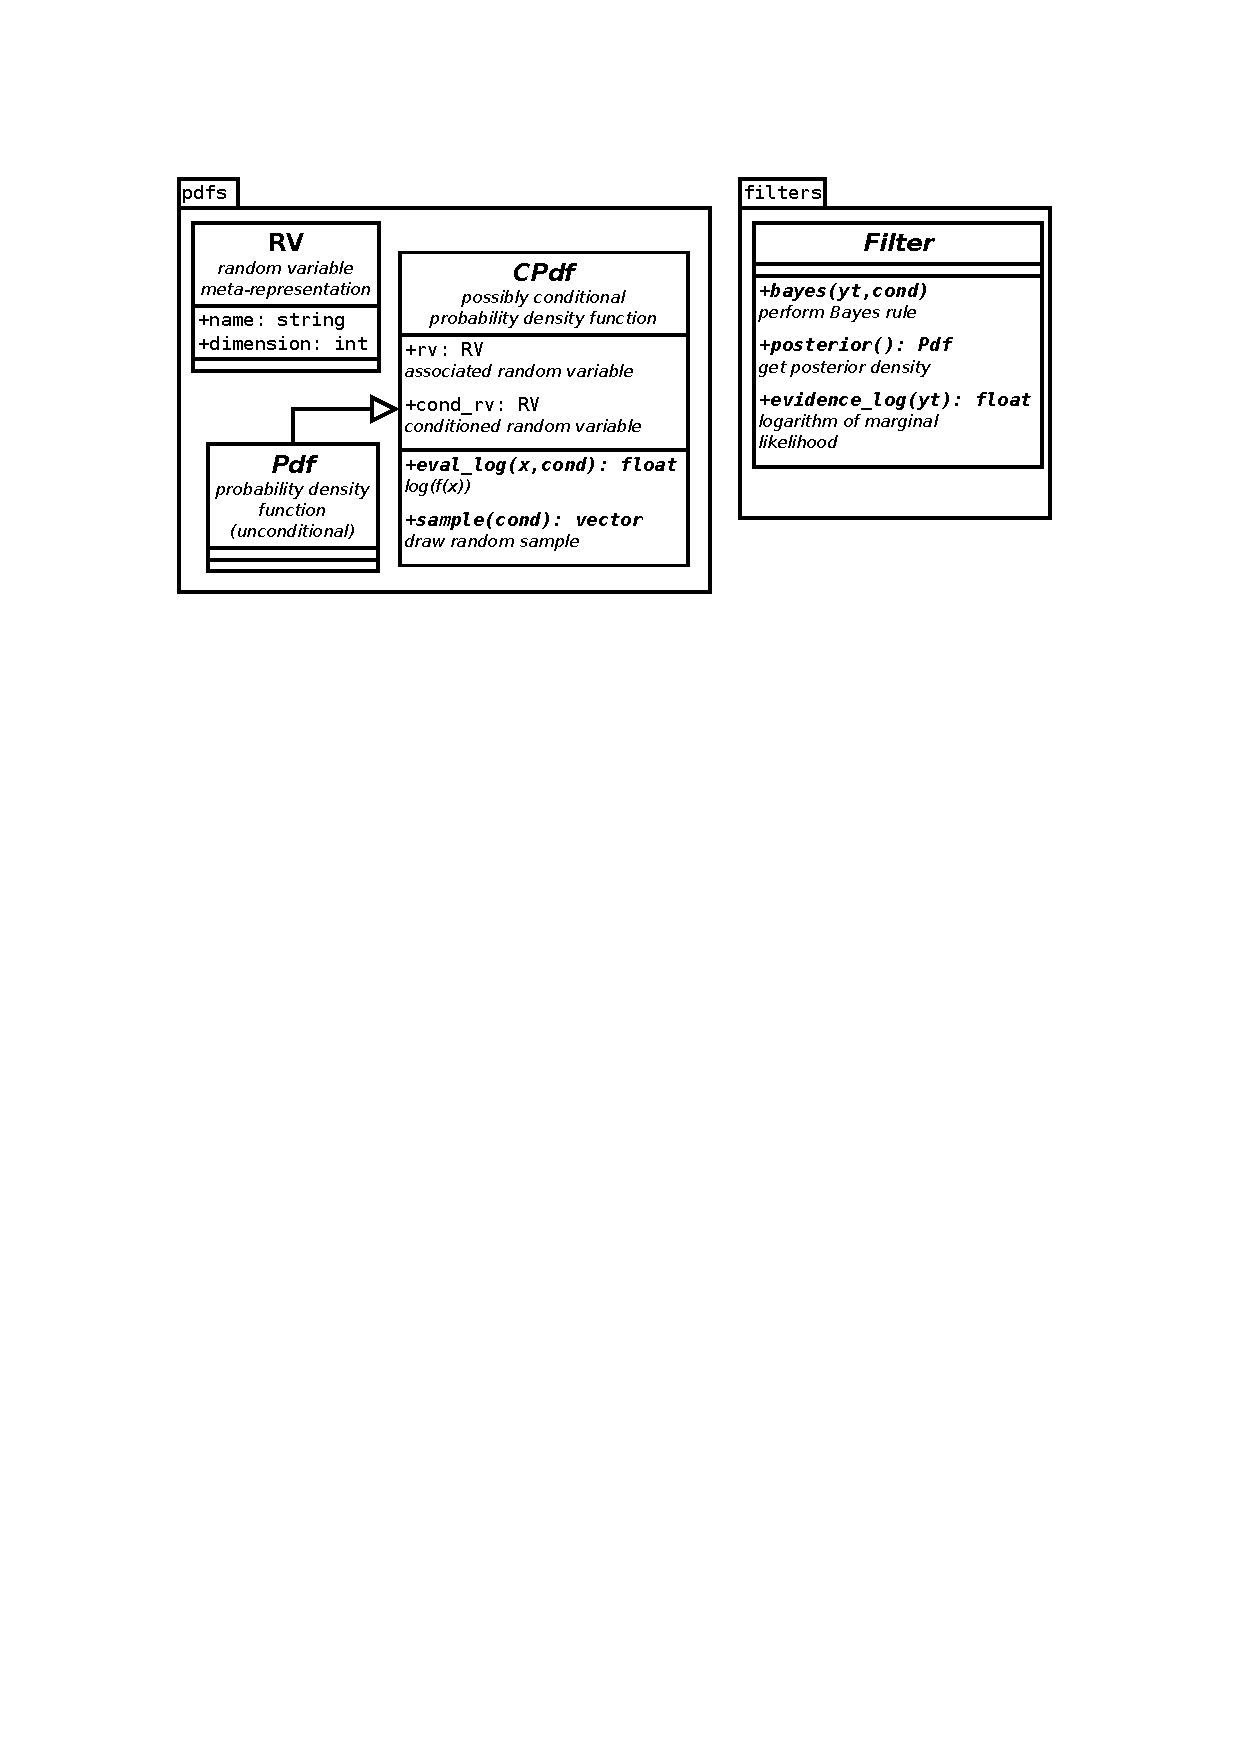
\includegraphics[width=\textwidth,keepaspectratio=true,clip=true,trim=3cm 196mm 3cm 3cm]{./diagrams/PyBayes.pdf}
	\vspace{-8mm}
	\caption{High-level overview of the PyBayes library; simplified}
\end{figure}

\subsection{Random Variable Meta-representation}

\begin{figure}[h]
	\centering
	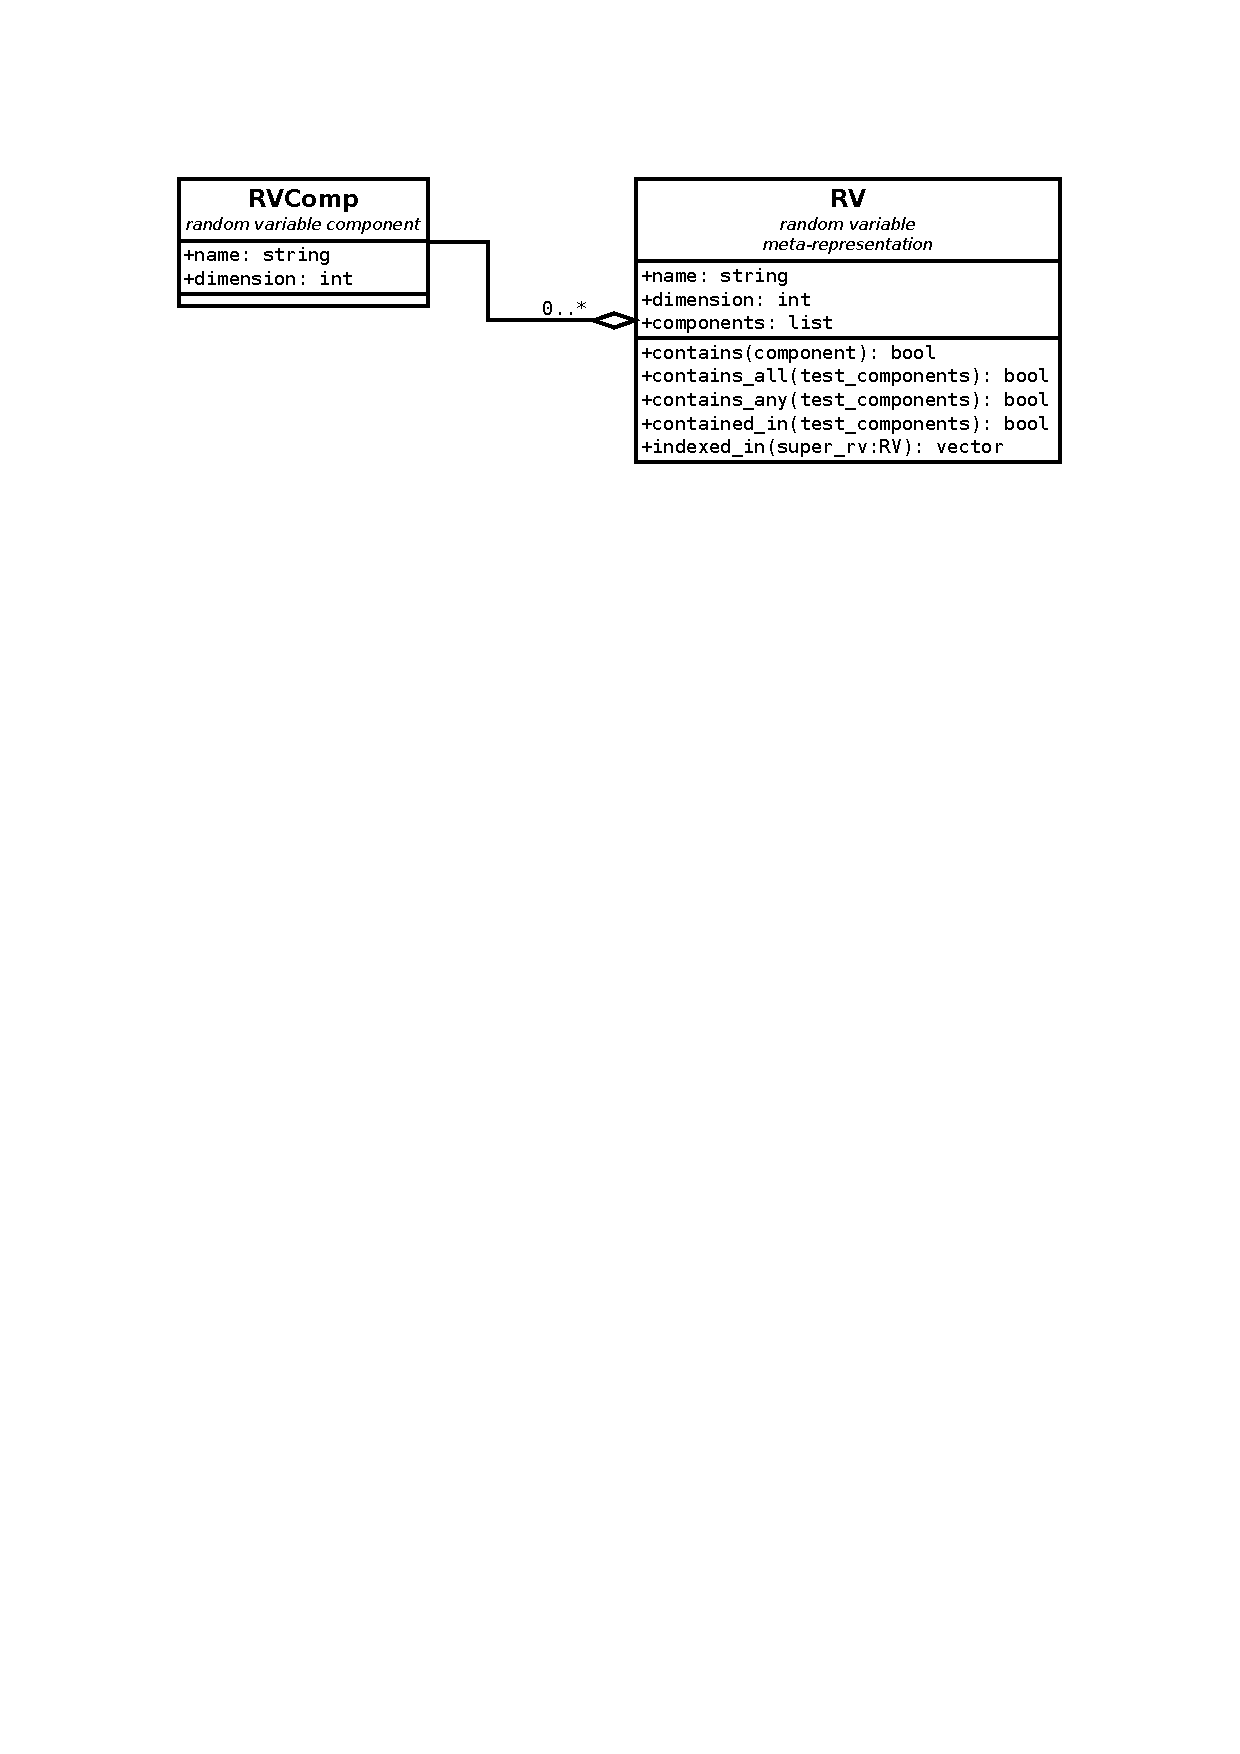
\includegraphics[width=\textwidth,keepaspectratio=true,clip=true,trim=3cm 218mm 3cm 3cm]{./diagrams/rvs.pdf}
	\vspace{-8mm}
	\caption{Class diagram of the random variable framework}
\end{figure}

Why it is needed (ref to ProdCPdf)

\subsection{Probability Density Function Prototypes}

\begin{figure}[h]
	\centering
	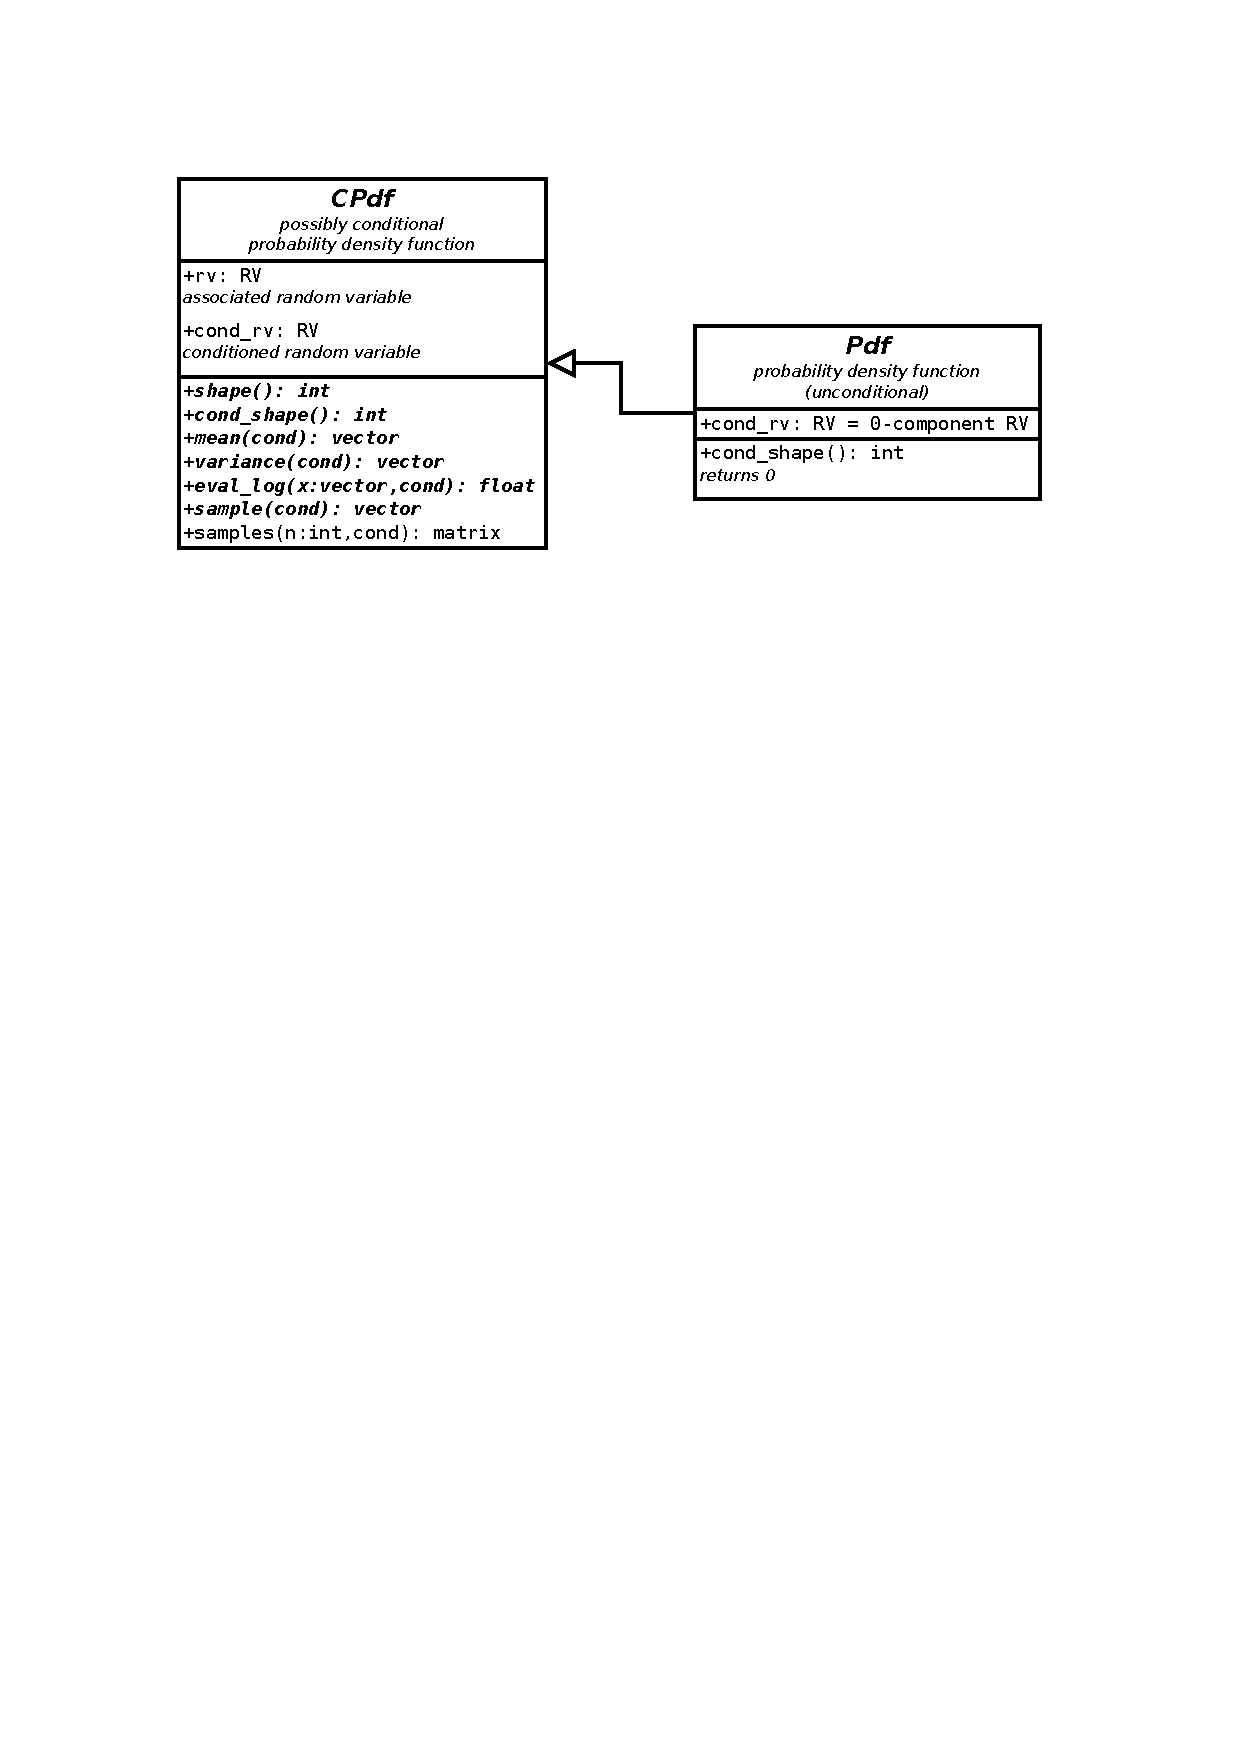
\includegraphics[width=\textwidth,keepaspectratio=true,clip=true,trim=3cm 204mm 3cm 3cm]{./diagrams/pdfs.pdf}
	\vspace{-8mm}
	\caption{Class diagram of the {\pdf} prototypes}
\end{figure}

... why pdfs from scipy weren't used

uniform pdf not mentioned elsewhere

\subsection{Gaussian Probability Density Functions}

\subsection{Empirical Probability Density Functions}

and their use in Particle filters

and in testing!

\subsection{Product Probability Density Functions}

\subsection{Bayesian Filters}

[proposed citation: \cite{Smi:05}]

UML

Nice graph of a run of a particle filter (Mirda has the plotting code)

similar of marginalized particle filter? (gausses would be plotted vertically)

[mention this:\cite{Smi:10}]

\subsection{Wrappers}

about numpy, linalg wrappers, Tokyo...

\section{Documentation, Testing and Profiling} \label{sec:PyBayesDocsTests}

TODO: move above Library Layout?

Documenting PyBayes using Sphinx, approach to documentation (mathematician-oriented), math in documentation

Testing - the separation of

- tests: test one class in isolation, quick, determinism (would be good, not achievable)

- stresses: test a great portion of code at once, run longer, non-determinism..

Note about coverage.py!!

Profiling python/cython - how, existing support in PyBayes

- how to correct profiling-induced overhead

\section{Performance Comparison with BDM} \label{sec:PyBayesPerformance}

[skip if in time press]
Python/Cython KalmanFilter, MATLAB oo / imperative / BDM

|see \autoref{fig:KF} (p. \pageref{fig:KF})|

\section{Future Plans}

jo?
